\documentclass[tikz,border=3mm]{standalone}

\usepackage{pgfplots}


\usetikzlibrary{decorations.pathreplacing}
\begin{document}
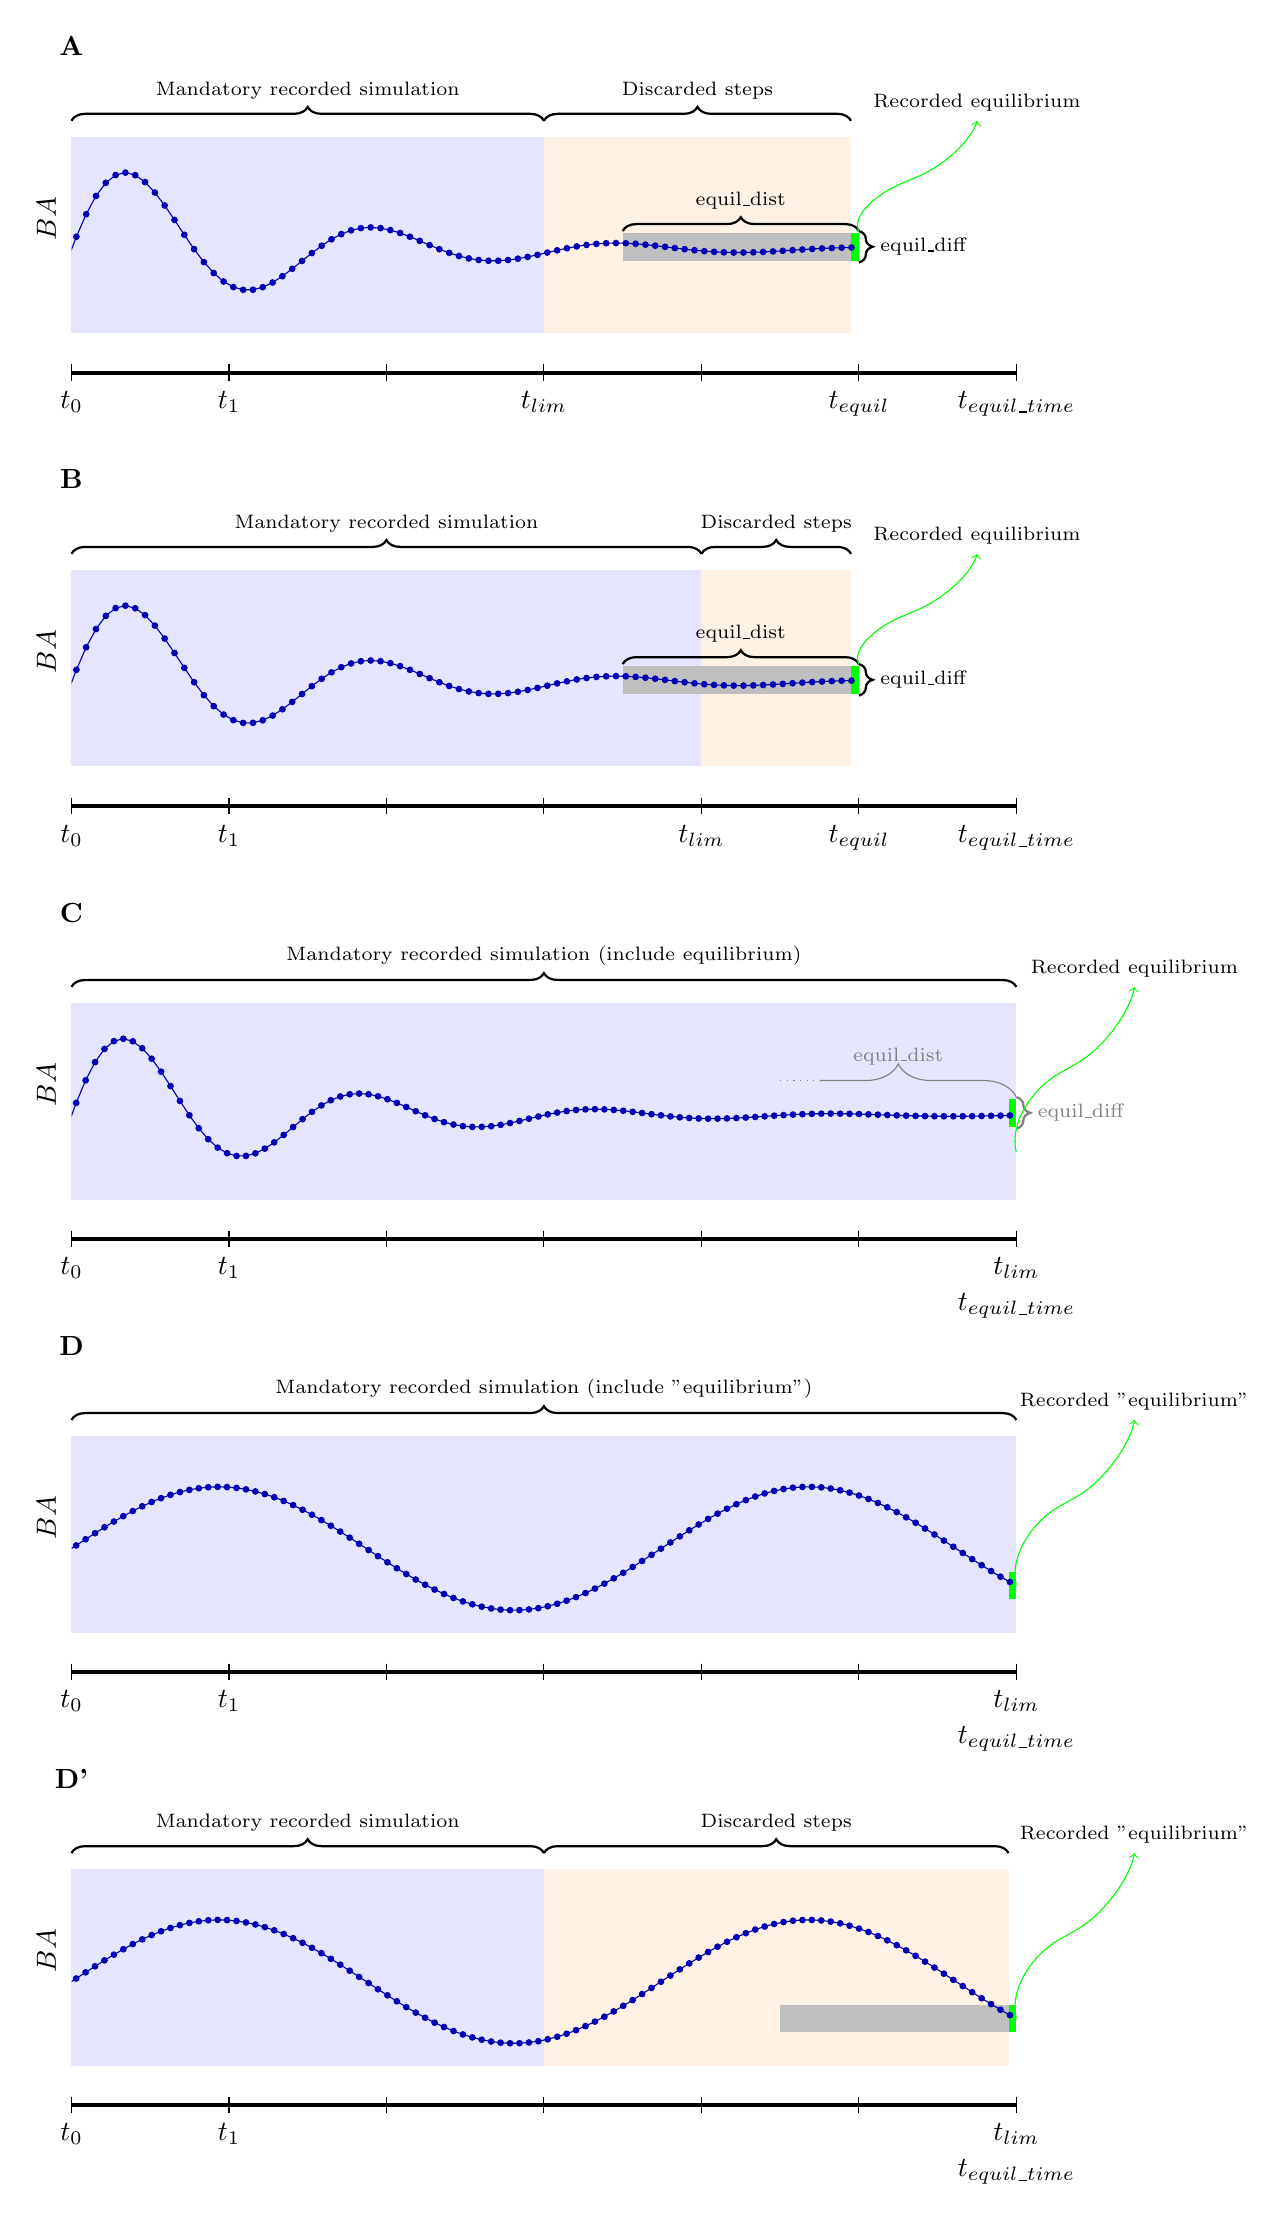
\begin{tikzpicture}

	\draw[ultra thick] (0,3) node[above= 25pt] {\textbf{A}};
	\draw[ultra thick] (0,0) -- (12,0);
	\draw[ultra thick] (0,0) node[below=3pt,thick] {$t_0$};
	\draw[ultra thick] (2,0) node[below=3pt,thick] {$t_1$};
	\draw[ultra thick] (6,0) node[below=3pt, thick] {$t_{lim}$};
	\draw[ultra thick] (12,0) node[below=3pt, thick] {$t_{equil\_time}$};
	\draw[ultra thick] (10,0) node[below=3pt, thick] {$t_{equil}$} {};
	\foreach \x in {0, 2,4,6,8,10, 12}
	\draw (\x cm,3pt) -- (\x cm,-3pt);

	\draw [thick ,decorate,decoration={brace,amplitude=5pt}] (0,3.2)  -- +(6,0)
	node [black,midway,above=4pt, font=\scriptsize] {Mandatory recorded simulation};
	%  \draw[green, line width=40pt](0,1) -- +(6,0);
	\fill[blue!10] (0,0.5) rectangle ++(6,2.5);
	\draw [thick ,decorate,decoration={brace,amplitude=5pt}] (6,3.2)  -- +(3.9,0)
	node [black,midway,above=4pt, font=\scriptsize] {Discarded steps};
	\fill[orange!10] (6,0.5) rectangle ++ (3.9,2.5);

	\draw [thick ,decorate,decoration={brace,amplitude=5pt}] (7,1.8)  -- +(3,0)
	node [black,midway,above=4pt, font=\scriptsize] {equil\_dist};
	\draw[lightgray, line width=10pt](7,1.6) -- +(2.9,0);
	\draw [thick ,decorate,decoration={brace,amplitude=5pt, mirror}] (10,1.4)  -- +(0,0.4)
	node [black,midway,right=4pt, font=\scriptsize] {equil\_diff};
	\draw[green, line width=10pt](9.9,1.6) -- +(.1,0);

	\begin{axis}[trig format plots=rad,axis lines=left, axis line style={draw=none},
			xtick=\empty,ytick=\empty, width=11.5cm,height=5.5cm,
			xmin=0, xmax=4, ymin=0, ymax=3, ylabel=$BA$, ylabel near ticks
		]
		\addplot[mark=*,mark size=1pt,color=blue!70!black,samples=200] {1.2+exp(-x)*sin(5*x)};
	\end{axis}

	\node[font=\scriptsize, above] at (11.5, 3.2) {Recorded equilibrium};
	\draw[green, ->] plot [smooth, tension=1] coordinates {(10, 1.8) (10.2,2.2) (11.1, 2.7) (11.5, 3.2)};


	\begin{scope}[yshift=-5.5cm]

		\draw[ultra thick] (0,3) node[above= 25pt] {\textbf{B}};
		\draw[ultra thick] (0,0) -- (12,0);
		\draw[ultra thick] (0,0) node[below=3pt] {$t_0$};
		\draw[ultra thick] (2,0) node[below=3pt] {$t_1$};
		\draw[ultra thick] (8,0) node[below=3pt] {$t_{lim}$};
		\draw[ultra thick] (10,0) node[below=3pt] {$t_{equil}$};
		\draw[ultra thick] (12,0) node[below=3pt] {$t_{equil\_time}$};
		\foreach \x in {0, 2,4,6,8,10, 12}
		\draw (\x cm,3pt) -- (\x cm,-3pt);

		\draw [thick ,decorate,decoration={brace,amplitude=5pt}] (0,3.2)  -- +(8,0)
		node [black,midway,above=4pt, font=\scriptsize] {Mandatory recorded simulation};
		%  \draw[green, line width=40pt](0,1) -- +(6,0);
		\fill[blue!10] (0,0.5) rectangle ++(8,2.5);
		\draw [thick ,decorate,decoration={brace,amplitude=5pt}] (8,3.2)  -- +(1.9,0)
		node [black,midway,above=4pt, font=\scriptsize] {Discarded steps};
		\fill[orange!10] (8,0.5) rectangle ++ (1.9,2.5);

		\draw [thick ,decorate,decoration={brace,amplitude=5pt}] (7,1.8)  -- +(3,0)
		node [black,midway,above=4pt, font=\scriptsize] {equil\_dist};
		\draw[lightgray, line width=10pt](7,1.6) -- +(2.9,0);
		\draw [thick ,decorate,decoration={brace,amplitude=5pt, mirror}] (10,1.4)  -- +(0,0.4)
		node [black,midway,right=4pt, font=\scriptsize] {equil\_diff};
		\draw[green, line width=10pt](9.9,1.6) -- +(.1,0);

		\begin{axis}[trig format plots=rad,axis lines=left, axis line style={draw=none},
				xtick=\empty,ytick=\empty, width=11.5cm,height=5.5cm,
				xmin=0, xmax=4, ymin=0, ymax=3, ylabel=$BA$, ylabel near ticks
			]
			\addplot[mark=*,mark size=1pt,color=blue!70!black,samples=200] {1.2+exp(-x)*sin(5*x)};
		\end{axis}

		\node[font=\scriptsize, above] at (11.5, 3.2) {Recorded equilibrium};
		\draw[green, ->] plot [smooth, tension=1] coordinates {(10, 1.8) (10.2,2.2) (11.1, 2.7) (11.5, 3.2)};


	\end{scope}

	\begin{scope}[yshift=-11cm]

		\draw[ultra thick] (0,3) node[above= 25pt] {\textbf{C}};
		\draw[ultra thick] (0,0) -- (12,0);
		\draw[ultra thick] (0,0) node[below=3pt,thick] {$t_0$};
		\draw[ultra thick] (2,0) node[below=3pt,thick] {$t_1$};
		\draw[ultra thick] (12,0) node[below=3pt, thick] {$t_{lim}$};
		\draw[ultra thick] (12,0) node[below=16pt, thick] {$t_{equil\_time}$};
		\foreach \x in {0, 2,4,6,8,10, 12}
		\draw (\x cm,3pt) -- (\x cm,-3pt);

		\draw [thick ,decorate,decoration={brace,amplitude=5pt}] (0,3.2)  -- +(12,0)
		node [black,midway,above=4pt, font=\scriptsize] {Mandatory recorded simulation (include equilibrium)};
		\fill[blue!10] (0,0.5) rectangle ++(12,2.5);
		\draw [gray, thick ,decorate,decoration={brace,amplitude=5pt, mirror}] (12,1.4)  -- +(0,0.4)
		node [gray,midway,right=4pt, font=\scriptsize] {equil\_diff};


		\draw[green, line width=10pt](11.9,1.6) -- +(.1,0);

		\begin{axis}[trig format plots=rad,axis lines=left, axis line style={draw=none},
				xtick=\empty,ytick=\empty, width=13.5cm,height=5.5cm,
				xmin=0, xmax=5, ymin=0, ymax=3, ylabel=$BA$, ylabel near ticks
			]
			\addplot[mark=*,mark size=1pt,color=blue!70!black,samples=200] {1.2+exp(-x)*sin(5*x)};
		\end{axis}

		\begin{scope}
			\clip(9.5, 3) rectangle (12, 0);
			\draw [gray, decorate,decoration={brace,amplitude=12pt}] (9,1.8) -- +(3,0)
			node [gray,midway,above=8pt, font=\scriptsize] {equil\_dist};
		\end{scope}
		\draw[gray, dotted] ([yshift=6pt]9, 1.8) -- ([yshift=6pt]9.5,1.8);

		\node[font=\scriptsize, above] at (13.5, 3.2) {Recorded equilibrium};
		\draw[green, ->] plot [smooth, tension=1] coordinates {(12, 1.1) (12.2,1.8) (13.1, 2.5) (13.5, 3.2)};

	\end{scope}

	\begin{scope}[yshift=-16.5cm]

		\draw[ultra thick] (0,3) node[above= 25pt] {\textbf{D}};
		\draw[ultra thick] (0,0) -- (12,0);
		\draw[ultra thick] (0,0) node[below=3pt,thick] {$t_0$};
		\draw[ultra thick] (2,0) node[below=3pt,thick] {$t_1$};
		\draw[ultra thick] (12,0) node[below=3pt, thick] {$t_{lim}$};
		\draw[ultra thick] (12,0) node[below=16pt, thick] {$t_{equil\_time}$};
		\foreach \x in {0, 2,4,6,8,10, 12}
		\draw (\x cm,3pt) -- (\x cm,-3pt);

		\draw [thick ,decorate,decoration={brace,amplitude=5pt}] (0,3.2)  -- +(12,0)
		node [black,midway,above=4pt, font=\scriptsize] {Mandatory recorded simulation (include "equilibrium")};
		\fill[blue!10] (0,0.5) rectangle ++(12,2.5);
		\draw[green, line width=10pt](11.9,1.1) -- +(.1,0);

		\begin{axis}[trig format plots=rad,axis lines=left, axis line style={draw=none},
				xtick=\empty,ytick=\empty, width=13.5cm,height=5.5cm,
				xmin=0, xmax=5, ymin=0, ymax=5, ylabel=$BA$, ylabel near ticks
			]
			\addplot[mark=*,mark size=1pt,color=blue!70!black,samples=200] {2+sin(2*x)};
		\end{axis}

		\node[font=\scriptsize, above] at (13.5, 3.2) {Recorded "equilibrium"};
		\draw[green, ->] plot [smooth, tension=1] coordinates {(12, 1.1) (12.2,1.8) (13.1, 2.5) (13.5, 3.2)};

	\end{scope}

	\begin{scope}[yshift=-22cm]

		\draw[ultra thick] (0,3) node[above= 25pt] {\textbf{D'}};
		\draw[ultra thick] (0,0) -- (12,0);
		\draw[ultra thick] (0,0) node[below=3pt,thick] {$t_0$};
		\draw[ultra thick] (2,0) node[below=3pt,thick] {$t_1$};
		\draw[ultra thick] (12,0) node[below=3pt, thick] {$t_{lim}$};
		\draw[ultra thick] (12,0) node[below=16pt, thick] {$t_{equil\_time}$};
		\foreach \x in {0, 2,4,6,8,10, 12}
		\draw (\x cm,3pt) -- (\x cm,-3pt);

		\draw [thick ,decorate,decoration={brace,amplitude=5pt}] (0,3.2)  -- +(6,0)
		node [black,midway,above=4pt, font=\scriptsize] {Mandatory recorded simulation };
		\fill[blue!10] (0,0.5) rectangle ++(6,2.5);
		\draw [thick ,decorate,decoration={brace,amplitude=5pt}] (6,3.2)  -- +(5.9,0)
		node [black,midway,above=4pt, font=\scriptsize] {Discarded steps};
		\fill[orange!10] (6,0.5) rectangle ++ (5.9,2.5);

		\draw[lightgray, line width=10pt](9,1.1) -- +(2.9,0);
		\draw[green, line width=10pt](11.9,1.1) -- +(.1,0);

		\begin{axis}[trig format plots=rad,axis lines=left, axis line style={draw=none},
				xtick=\empty,ytick=\empty, width=13.5cm,height=5.5cm,
				xmin=0, xmax=5, ymin=0, ymax=5, ylabel=$BA$, ylabel near ticks
			]
			\addplot[mark=*,mark size=1pt,color=blue!70!black,samples=200] {2+sin(2*x)};
		\end{axis}

		\node[font=\scriptsize, above] at (13.5, 3.2) {Recorded "equilibrium"};
		\draw[green, ->] plot [smooth, tension=1] coordinates {(12, 1.1) (12.2,1.8) (13.1, 2.5) (13.5, 3.2)};

	\end{scope}

\end{tikzpicture}

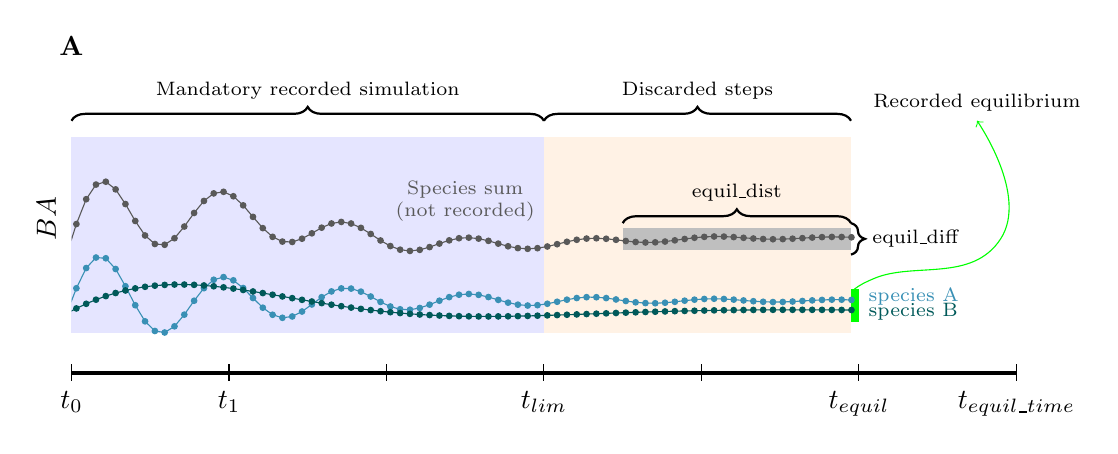
\begin{tikzpicture}

	\draw[ultra thick] (0,3) node[above= 25pt] {\textbf{A}};
	\draw[ultra thick] (0,0) -- (12,0);
	\draw[ultra thick] (0,0) node[below=3pt,thick] {$t_0$};
	\draw[ultra thick] (2,0) node[below=3pt,thick] {$t_1$};
	\draw[ultra thick] (6,0) node[below=3pt, thick] {$t_{lim}$};
	\draw[ultra thick] (12,0) node[below=3pt, thick] {$t_{equil\_time}$};
	\draw[ultra thick] (10,0) node[below=3pt, thick] {$t_{equil}$} {};
	\foreach \x in {0, 2,4,6,8,10, 12}
	\draw (\x cm,3pt) -- (\x cm,-3pt);

	\draw [thick ,decorate,decoration={brace,amplitude=5pt}] (0,3.2)  -- +(6,0)
	node [black,midway,above=4pt, font=\scriptsize] {Mandatory recorded simulation};
	%  \draw[green, line width=40pt](0,1) -- +(6,0);
	\fill[blue!10] (0,0.5) rectangle ++(6,2.5);
	\draw [thick ,decorate,decoration={brace,amplitude=5pt}] (6,3.2)  -- +(3.9,0)
	node [black,midway,above=4pt, font=\scriptsize] {Discarded steps};
	\fill[orange!10] (6,0.5) rectangle ++ (3.9,2.5);

	\draw [thick ,decorate,decoration={brace,amplitude=5pt}] (7,1.9)  -- +(2.9,0)
	node [black,midway,above=4pt, font=\scriptsize] {equil\_dist};
	\draw[lightgray, line width=8pt](7,1.7) -- +(2.9,0);
	\draw [thick ,decorate,decoration={brace,amplitude=5pt, mirror}] (9.9,1.5)  -- +(0,0.4)
	node [black,midway,right=4pt, font=\scriptsize] {equil\_diff};
	\draw[green, line width=12pt](9.9,0.85) -- +(.1,0);

	\begin{axis}[trig format plots=rad,axis lines=left, axis line style={draw=none},
			xtick=\empty,ytick=\empty, width=11.5cm,height=5.5cm,
			xmin=0, xmax=4, ymin=0, ymax=6, ylabel=$BA$, ylabel near ticks
		]
		\addplot[mark=*,mark size=1pt,color=cyan!70!black,samples=200] {1.4+exp(-x)*sin(10*x)};
		\addplot[mark=*,mark size=1pt,color=teal!70!black,samples=200] {1.2+exp(-x)*sin(2*x)};
		\addplot[mark=*,mark size=1pt,color=gray!70!black,samples=200] {1.4+exp(-x)*sin(10*x)+ 1.2+exp(-x)*sin(2*x)};
	\end{axis}

	\node[font=\scriptsize, above] at (11.5, 3.2) {Recorded equilibrium};
	\draw[green, ->] plot [smooth, tension=1] coordinates {(10, 0.95) (10.2,1.2) (11.8, 1.7) (11.5, 3.2)};

	\node[font=\scriptsize, right, cyan!70!black] at (10, 0.97) {species A};
	\node[font=\scriptsize, right, teal!70!black] at (10, 0.78) {species B};
	\node[font=\scriptsize, align= center, above, gray!70!black] at (5, 1.8) {Species sum \\(not recorded)};

\end{tikzpicture}

\end{document}